
\begin{lemma} 
    \label{Lemma1}
    Consider three events $e$,$d$ and $k$. \\

    If
        \[
            \cons{e}{d} \ \wedge \ \reln{e}{ao}{d} \ \wedge \
            (
                (\et{d}{uo}) \ \vee \
                (\et{d}{sc} \ \wedge \ \event{d}{W})
            )
        \]
        
    then,
        \[
            \reln{k}{hb}{d} \Rightarrow \reln{k}{hb}{e}.
        \]
      
    When we have two consecutive events \textit{e} and \textit{d} which are one after the other (i.e. $\reln{e}{ao}{d}$), we can use \textit{transitive property} of $\stck{_{hb}}$ to infer that any event \textit{k} that \textit{happens before} \textit{e}, also \textit{happens before} \textit{d}. However, is it possible to derive that the event \textit{k happens before e} using the evidence that \textit{k happens before d} ? This lemma states the condition when this is true.
    
\end{lemma}

%An alternative short proof 
\begin{proof}
    
    We will divide the proof for this into two cases, based on what event $d$ is. For both cases, we have the following to be true :
    
    \begin{align*}
        cons(e,d) \ \wedge \ \reln{e}{ao}{d}.
        \tag{0}
        \label{l10}
    \end{align*}
        
    In the first case, we have $\et{d}{uo}$. From Def \ref{Dir} and Def \ref{Cons}, we have for any event $k$
    \begin{align*}
        dir(k,d) \Rightarrow cons(k,d).
    \end{align*}
        
    From (\ref{l10}), we have $k=e$ satisfying the above property with $d$. 
    Because $\stck{_{ao}}$ is a total order, $e$ will be the only event. Thus, for any other $k \neq e$, we have 
    
    \begin{align*}
        \reln{k}{hb}{d} \Rightarrow \reln{k}{hb}{d}.
    \end{align*}
    
    In the second case, we have 
    \[
        \et{d}{sc} \wedge d\!\in\!W.
        \tag{4}
        \label{l14}
    \]
    
    Thus, from Def \ref{Dir} and Def \ref{Cons}, for any event $k$, we have 
    \[
        dir(k,d) \Rightarrow cons(k,d).
    \]
    
    From (\ref{l14}), event $e$ satisfies the above.
    Though there could be direct \textit{happens-before} relation with some event $k$ from another \textit{agent}, from Def \ref{Dir} these are only relations satisfying $dir(d,k)$. Thus, we can once again infer that for any $k \neq e$ 
    
    \[
        \reln{k}{hb}{d} \Rightarrow \reln{k}{hb}{d}.
    \]
    
    The following figure summarizes the intuition behind both cases: 
    
    \begin{figure}[H]
        \centering
        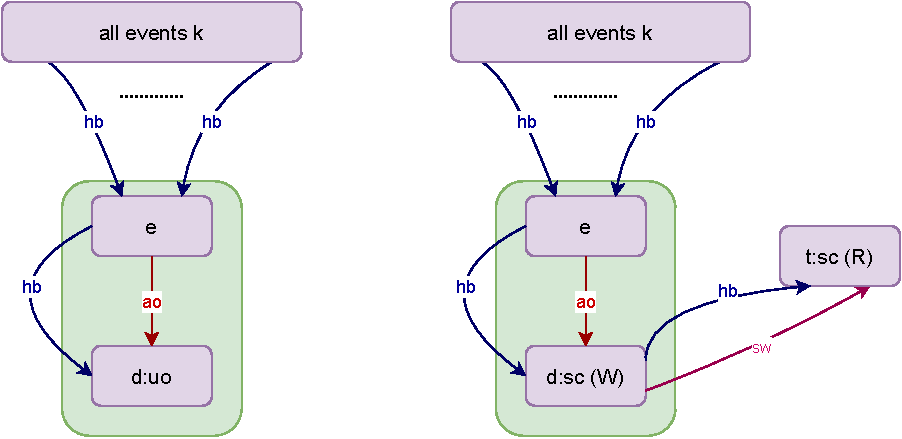
\includegraphics[scale=0.7]{5.InstructionReordering/3.Lemmas/Lemma1.pdf}
        \caption{Left figure is for first case and right one for the second}
        \label{fig:my_label}
    \end{figure}
    
\end{proof}

%---------------------------------------------------------------------------------------------------------------    

%SHORTER VERSION OF PROOF WITHOUT THE ENGLISH EXPLAINATION IN THE MIDDLE. DISCUSS AND DECIDE ON WHICH FORM IS BETTER
\begin{lemma}
    \label{Lemma2}
    Consider three events $e$, $d$ and $k$ \\

    If
        
        \[
            \cons{e}{d} \ \wedge \ \reln{e}{ao}{d} \ \wedge \
            (
                (\et{e}{uo}) \ \vee \
                (\et{e}{sc} \ \wedge \ \event{e}{R})
            )
        \]
        
    then,
        \[
            \reln{e}{hb}{k} \Rightarrow \reln{d}{hb}{k}.
        \]

 When we have two consecutive events \textit{e} and \textit{d} which are one after the other (i.e. $\reln{e}{ao}{d}$), we can use \textit{transitive property} of $\stck{_{hb}}$ to infer that any event \textit{k} that \textit{happens after} \textit{d}, also \textit{happens after} \textit{e}. However, is it possible to derive that the event \textit{k happens after d} using the evidence that \textit{k happens after e} ? This lemma states the condition when this is true.

\end{lemma}

%An alternative proof for this 
\begin{proof}
    
    Just like the proof for the previous lemma, we will divide the proof for this into two cases, based on what event $e$ is. Again, for both cases, we have the following to be true:
    
    \[
        cons(e,d) \ \wedge \reln{e}{ao}{d}.
        \tag{0}
        \label{l20}
    \]

   In the first case, we have $\et{e}{uo}$. From Def \ref{Dir} and Def \ref{Cons}, we have for any event $k$
   \[
        dir(e,k) \Rightarrow cons(e,k).
   \]
   
   From (\ref{l10}), we have $k=d$ satisfying the above property with $e$. 
   Because $\stck{_{ao}}$ is a total order, $d$ would be the only such event. 
   Thus, for any other event $k \neq d$, we can infer,
   
   \[
        \reln{e}{hb}{k} \Rightarrow \reln{d}{hb}{k}.
   \]
   
    In the second case, we have 
    \[
        \et{e}{sc} \wedge e\!\in\!R.
        \tag{4}
        \label{l24}
    \]
    
    Thus, from Def \ref{Dir} and Def \ref{Cons}, for any event $k$, we have 
    \[
        dir(e,k) \Rightarrow cons(e,k).
    \]
    
    From (\ref{l24}), we have event $k=d$ satisfying the above property with $e$  
    Though there could be direct \textit{happens-before} relation with some event $k$ from another \textit{agent}, from Def \ref{Dir} these are only relations satisfying $dir(k,e)$. Thus, we can infer that for any $k \neq d$ 
    
    \[
        \reln{e}{hb}{k} \Rightarrow \reln{d}{hb}{k}.
    \]
    
    The following figure summarizes the intuition behind both cases: 
    
    \begin{figure}[H]
        \centering
        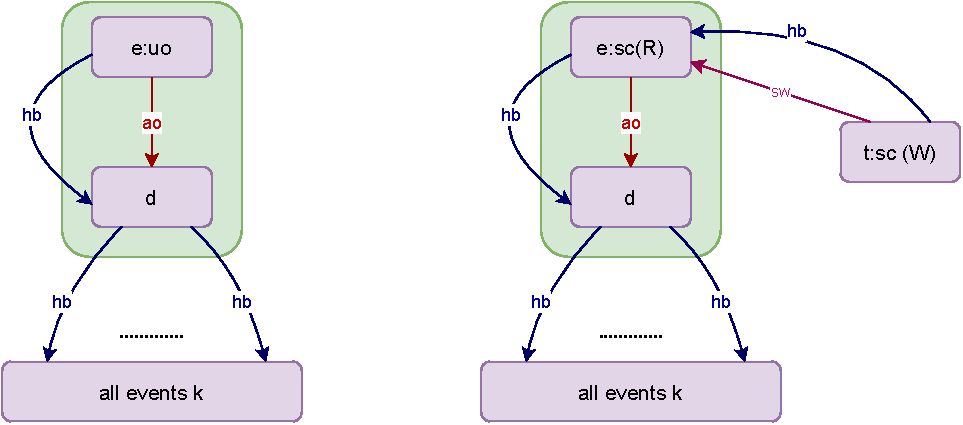
\includegraphics[scale=0.7]{5.InstructionReordering/3.Lemmas/Lemma2.pdf}
        \caption{Left figure is for first case and right one for the second}
        \label{fig:my_label}
    \end{figure}

\end{proof}

%------------------------------------------------------------------------------
